
% JuliaCon proceedings template
\documentclass{juliacon}

\usepackage{amsmath}
\usepackage{tabularx}
\usepackage[strings]{underscore}

% Defining some useful symbols
\DeclareMathOperator{\Cl}{Cl}

\newcommand{\ClR}[1]{\Cl_{#1}\left(\mathbb{R}\right)}
\newcommand{\ClC}[1]{\Cl_{#1}\left(\mathbb{C}\right)}

\setcounter{page}{1}

\begin{document}

% **************GENERATED FILE, DO NOT EDIT**************

\title{CliffordNumbers.jl: a Julia package for numeric primitives for geometry}

\author[1, 2]{Brandon S. Flores}
\author[2]{Victor M. Zavala}
\affil[1]{Department of Chemistry, University of Wisconsin-Madison}
\affil[2]{Department of Chemical and Biological Engineering, University of Wisconsin-Madison}

\keywords{Julia, Geometry, Geometric algebra, Clifford algebra, Exterior algebra, Numerical libraries}

\hypersetup{
pdftitle = {CliffordNumbers.jl: a Julia package for numeric primitives for geometry},
pdfsubject = {JuliaCon 2025 Proceedings},
pdfauthor = {Brandon S. Flores, Victor M. Zavala},
pdfkeywords = {Julia, Geometry, Geometric algebra, Clifford algebra, Exterior algebra, Numerical libraries},
}



\maketitle

\begin{abstract}

This is a guide for authors who are preparing papers for JuliaCon using the \LaTeX{} document
preparation system and the \verb|juliacon|  class file.

\end{abstract}

\section{Introduction}

One of the great challenges of modeling physical systems is the treatement of dimensions.
Historically, two major conventions have been used to model 3D space.
In 1843, William Rowan Hamilton famously inscribed the formula $i^2 = j^2 = k^2 = ijk = -1$  into the stone of Brougham Bridge with a pocket knife, defining the quaternions.
Quaternions can encode both scalar quantities and three-dimensional vectors in a single object, and they permit addition, multiplication, and their inverses.
Although the quaternions immediately found use in the physical sciences, notably in Maxwell's first publication of his famous equations, they were also considered unwieldy: Maxwell originally published 20 equations instead of the four we know today.
Part of this unwieldiness stems from the noncommutativity of quaternion multiplication, but this property is necessary to describe rotations in three dimensions.
More troubling was that 3D vectors would always have negative squares, which requires careful manipulation of signs to ensure that quantities are correctly computed.

The deficiencies of quaternions led Josiah Willard Gibbs to develop a new formalism, vector algebra, which is the dominant formalism in all but a few niche applications today.
Rather than a single quaternion product, vector algebra uses two products, the dot and cross product, splitting the commutative and anticommutative components of the quaternion product into two different operations.
However, vector algebra is not free of unwieldiness, either, particularly with the cross product.
The cross product of two vectors does not transform like the input vectors under a reflection or other transformation that reverses the orientation of the space.
For clarity, the output of the cross product is often called a \textit{pseudovector}, and the dot product of a pseudovector with a vector (as in the triple product) is called a \textit{pseudoscalar}.
The vector algebra formalism requires these distinctions to correctly describe how multidimensional quantities transform.

Today, most physics literature is written in the language of vector calculus, a combination of calculus and vector algebra.
By contrast, quaternions see relatively little practical use, with the most notable exception being the description of 3D rotations.
However, both quaternions and vector algebra also share one glaring deficiency: they are limited to describing 3D space.
This is obvious from the limited size of quaternions, but even vector algebra is deficient in this regard without combining it with matrix algebra.
It is possible to generalize the cross product to an $n-1$-ary operator on $n$-dimensional vectors, but this means that the binary nature of the cross product is dependent on three dimensions.
(A seven-dimensional generalization exists, but does not satisfy the Jacobi identity.)\cite{lounesto2001clifford}

While Hamilton's quaternions and Gibbs' vector algebra battled for dominance in the scientific community, a third formalism developed in the shadows.
In 1844, Hermann Grassmann introduced \textit{Ausdehnungslehre} (\textit{Theory of Extension}), which we call \textit{exterior algebra} today.
This algebra combines $k$ $d$-dimensional vectors into new objects called \textit{$k$-vectors} (with the \textit{grade}, $k$, ranging from 0 to $d$), with $\binom{d}{k}$ components, using a new operation, the \textit{wedge product} ($\wedge$).
With the wedge product, objects of any dimension from 0 to $d$ residing in a $d$-dimensional space can be rigorously described.
In three dimensions, the wedge product of two vectors is calculated exactly as the cross product is, but the result is a not an ordinary vector, but a $2$-vector (or bivector).
This distinction explains why axial vectors and pseudovectors transform differently in the vector calculus formalism: axial vectors are $1$-vectors, and pseudovectors are $2$-vectors (or more generally $\left(d-1\right)$-vectors in $d$ dimensions).

In 1878, William Kingdon Clifford, familiar with the work of Hamilton and Grassmann realized that the "vector" components of quaternions actually transformed like the bivectors of a three-dimensional exterior algebra.
He then constructed a new family of algebras, which he called \textit{$n$-way geometric algebras}, which extended the exterior algebra to include quaternion-like constructions which worked in any number of dimensions.
Today, these algebras are called \textit{Clifford algebras} in his honor.

Clifford's geometric algebra, as he formulated it, faded into obscurity.
Notably, Paul Dirac used the geometric algebra of spacetime in his derivation of his eponymous equation, but phrased it in the language of matrices.
Most literature on Clifford algebras uses the matrix-based formalism of representation theory, unlike Clifford's approach which treated Clifford algebras as a hypercomplex number system.
David Hestenes advocated for a return to Clifford's original geometric approach, and used this framework to develop new approaches to geometric and physical problems.\cite{CA2GC}
Although geometric algebra is still a niche formalism today, there has been a recent resurgence of interest in the topic: in part due to potential increases in computational efficiently, but primarily due to the conceptual and pedagogical clarity of the approach.

\subsection*{Statement of need}

The first computational tool we turn to when solving multidimensional problems is usually numerical linear algebra.
Numerous libraries exist to efficiently implement fundamental matrix and vector operations efficiently and with high numerical stability.
However, linear algebra may not be the best mathematical tool for phrasing a solution to a problem in low-dimensional geometry, and in some cases it may be an inferior approach for reasons that are not immediately obvious.
A prime example is implementing 3D rotations and reflections: while they can be composed and performed with matrix-vector multiplication, it has suboptimal efficiency, is not numerically stable, and can introduce shearing that does not respect the orthonormality of the space.

CliffordNumbers.jl aims to provide an implementation of geometric algebras that is fast and easy to use, with a well-documented implementation that can be used as a reference for others who wish to efficiently implement the fundamental operations of geometric algebra.
It supports algebras of arbitrary dimension, but the most common anticipated use cases are algebras of low dimensionality, which can take advantage of Julia's compiler infrastructure to produce highly optimized code for common numeric types, including the use of SIMD instructions.
Although it is possible to use matrix representations to perform all of the operations of a Clifford algebra, it is rare to require an explicit representation of all linearly independent components, so CliffordNumbers.jl provides small types for handling those cases efficiently.
All types representing elements of a Clifford algebra provided by the package subtype \texttt{Number} rather than \texttt{Array}, allowing them to interoperate seamlessly with existing Julia \texttt{Number} types and operations, including the type promotion mechanism.

\section{Mathematical background}

Formally, a \textit{Clifford algebra} $\Cl\left(V, \operatorname{Q}\right)$ is a unital associative algebra over the vector space $V$ and field $K$ and quadratic form $\operatorname{Q}: V \to K$.
Specifically, it is the quotient of the tensor algebra over $V$, $T(V) = \bigoplus_{x = 0}^{\infty} T^x V$, with respect to the two-sided ideal $v \otimes v - \operatorname{Q}\left(v\right) 1$ for all $v \in V$.
For most readers, this definition will likely not be informative without further context.

We start with an $n$-dimensional vector space $V$, and define the quadratic form as the dot product of vectors with themselves: $\operatorname{Q}\left(v\right) = v \cdot v$.
The tensor algebra $T(V)$ is the set of all tensor products of elements of $V$.
Each vector in $V$ is a $1$-tensor, and the tensor product of $k$ elements is a $k$-tensor, with the empty product ($0$-tensors) being scalars $K$.
The space of tensors of grade $k$ over $V$, $T^k V$, has dimension $n^k$.

With this, we construct the exterior algebra over $V$, $\bigwedge\left(V\right)$, by taking the quotient of $T(V)$ with respect to the two-sided ideal $v \otimes v$.
All tensors of the form $v \otimes v$ are symmetric tensors, and the two-sided ideal eliminates that contribution from the tensor product.
This tell us that the product of the exterior algebra, the \textit{wedge product} ($u \wedge v$), is the antisymmetric component of the tensor product $u \otimes v$.
It also tells us that the wedge product of linearly dependent of vectors is zero.
This limits the grades of $\bigwedge\left(V\right)$ to values between $0$ and $n$.

The subspaces of $\bigwedge\left(V\right)$ with grade $k$ are denoted $\bigwedge^{k}\left(V\right)$, and their elements are called $k$-vectors, which have $\binom{n}{k}$ components.
A general $k$-vector is a linear combination of \textit{$k$-blades}, which are generated by the wedge products of $k$ $1$-vectors.
$k$-blades correspond to oriented regions spanned by the $1$-vectors which generated them, and represent primitive geometric objects.
For all exterior algebras, scalars, vectors, $n-1$-vectors, and $n$-vectors are always blades.
Therefore, all $k$-vectors are blades in spaces of dimension 3 and below.
We can also sum of $k$-vectors of different grades, producing \textit{multivectors}.

We can now construct the Clifford algebra as a modification of the exterior algebra.
The quadratic form $\operatorname{Q}$ is simply the dot product of vectors with themselves: $\operatorname{Q}\left(v\right) = v \cdot v$.
With this, we modify the ideal we used to generate the exterior product from $T(V)$ to $v \otimes v - \operatorname{Q}\left(v\right) 1$.
Instead of eliminating the symmetric component of $u \times v$, we replace it a scalar, $u \cdot v$.
The \textit{Clifford product} or \textit{geometric product} of two $1$-vectors (denoted without an operator, $u v$) can now be described succinctly:
\begin{flalign}
    u v & = u \cdot v + u \wedge v
\end{flalign}
While this formula only holds for a very specific case, it may be used to derive the geometric product formula for arbitrary multivectors.

Like $k$-blades in the exterior algebra, we use the term $k$-versor to refer to geometric products of $1$-vectors.
Each versor corresponds to an isometry of space, with $1$-versors corresponding to reflections, $2$-versors to rotations, and $n$-versors to inversions, all combined with a scale factor proportional to the magnitude of the versor.
In general, $k$-versors are the sum of blades with grades of the same parity as $k$, allowing us to classify versors as \textit{even} and \textit{odd}.
The preservation of grade parity by the Clifford product indicates that Clifford algebras are $\mathbb{Z}_2$-graded algebras.

\subsection{Grade operations}

Geometric algebras admit a few special operations that manipulate the signs of components of different grades.

The \textit{main involution}, or \textit{grade involution} of $M$, $M^*$, reverses the signs of all components of odd grade.
This is equivalent to a spatial inversion, and changes the orientation of a blade if both the blade and algebra has odd dimension.
The \textit{reverse} of $M$, $M^\dagger$, reverses the signs of all components whose grade \textit{modulo} 2 is odd.
This operation is analogous to complex conjugation or the matrix adjoint in that it reverses the order of multiplication:
\begin{flalign}
a^\dagger b^\dagger & = \left(b a\right)^\dagger
\end{flalign}
The \textit{Clifford conjugate} of $M$ is the composition of the main involution and the reverse.

In CliffordNumbers.jl, we overload \texttt{Base.reverse} and \texttt{Base.adjoint} for the reverse, and we overload \texttt{Base.conj} for the Clifford conjugate.
This choice was made to align with the behavior of \texttt{Base.adjoint} for matrix multiplication, and to ensure that two possible representations of quaternions in CliffordNumbers.jl (either all elements of $\ClR{0,2,0}$ or the even elements of $\ClR{3,0,0}$) behave identically.

\subsection{Arithmetic operations}

As with ordinary vectors, all elements of a Clifford algebra can be added to each other and scaled by some scalar, so the usual \texttt{+}, \texttt{-}, \texttt{*}, and \texttt{/} operators behave as expected.
The geometric product also uses the \texttt{*} operator, and the wedge product may performed with either the $\wedge$ operator or the \texttt{wedge} function.

While the quadratic form, geometric product and wedge product are fundamental to geometric algebra, geometric algebras also admit other kinds of operations useful in expressing geometric transformations.

\subsubsection{Exponentiation}

The square of a multivector is defined as the geometric product of a multivector with itself:
\begin{flalign}
a^2 & = a a
\end{flalign}
Because the wedge product of any blade with itself is zero, the square of a blade is always a scalar.
In algebras with 3 or fewer dimensions, all $k$-vectors are blades, so they always have scalar squares.
But this does not hold in any space of higher dimension:
the wedge product of the $2$-blade $e_1 e_2 + e_3 e_4$ with itself is not zero, but $2 e_1 e_2 e_3 e_4$, since $e_1 e_2$ and $e_3 e_4$ have no factors in commmon.
Therefore, the square of this blade must have a non-scalar factor, and it is $2\left(-1 + e_1 e_2 e_3 e_4\right)$.

From this, all positive integer powers can be defined in terms of the geometric product.
CliffordNumbers leverages \texttt{Base.literal_pow} to convert the result of exponentiation to a type of minimum size.

Additionally, it is also possible to define a natural exponential of a blade $b$ using Taylor series, analogous to complex and quaternion exponentiation.
This can be broken down depending on the sign of the square of the blade:
\begin{flalign}
e^b = \sum_{n = 1}^{\infty} \frac{1}{n!} b^n 
    & = \begin{cases}
        \cos  \left|b\right| + b \sin  \left|b\right|, & b^2 < 0 \\
        \cosh \left|b\right| + b \sinh \left|b\right|, & b^2 > 0 \\
        1 + b,                                         & b^2 = 0 \\
    \end{cases}
\end{flalign}
Due to the noncommutativity of geometric algebras, the natural exponential of arbitrary multivectors cannot be broken down into a simple sum using the defining property of scalar exponentiation, $e^{a+b} = e^a e^b$.

In the vast majority of cases, the objects to be exponentiated are even multivectors, particularly $2$-blades, as these are taken to represent rotations or other types of fundamental transformations, as we will see later.

\subsubsection{Inverses and division}

Every blade and versor with nonzero square has an inverse:
\begin{flalign}
a & = \frac{1}{a^2} a^\dagger
\end{flalign}
However, arbitrary elements of a geometric algebra do not necessarily have an inverse, and may instead have zero divisors.
CliffordNumbers.jl overloads \texttt{inv} with a checked inverse function that throws a \texttt{CliffordNumbers.InverseException} if the input does not have a defined inverse.

Because geometric algebras are not commutative, it is also necessary to distinguish between left and right division, and we overload the right division operator \texttt{\textbackslash}, which is already used for matrix operations, to allow these operations to be clearly distinguished.

\subsubsection{Duality}

The grade $n$ element of an $n$-dimensional geometric algebra, or \textit{pseudoscalar} (generically written as $I$), has a special property: multiplying a $k$-vector by the pseudoscalar produces a $n-k$-vector.
This allows us to define the \textit{dual} of a multivector $a$:
\begin{flalign}
\operatorname{dual}\left(a\right)
    & = a I^{-1}
\end{flalign}
The dual can be extended to any multivector through the linearity of the geometric product.
The reason we use the inverse of the pseudoscalar here is so that we satisfy the following property:
\begin{flalign}
a \operatorname{dual}\left(a\right)^{-1} & = I
\end{flalign}
The inverse of $I$ depends on the dimension of the algebra $n$ as well as the quadratic form:
\begin{flalign}
I^{-1} & = \left(-1\right)^{\lfloor \frac{1}{2} n + q \rfloor}I
\end{flalign}
where $q$ is the number of dimensions with negative square.

However, we can extend our idea of duality if we base it on the wedge product.
For a basis blade $e$, the \textit{right complement} $\overline{e}$ and \textit{left complement} $\underline{e}$ are the basis blades that satisfy the following relations:
\begin{flalign}
e \wedge \overline{e}
    & = I \\
\underline{e} \wedge e
    & = I
\end{flalign}
As with the pseudoscalar dual, these can be extended by linearity to all multivectors of a geometric algebra.

In CliffordNumbers.jl, the function \texttt{pseudoscalar(x)} generates the pseudoscalar of the algebra \texttt{x} belongs to.
The left contraction and right contraction are provided with the functions \texttt{left_contraction} and \texttt{right_contraction}, respectively.

\subsubsection{Regressive product}
The regressive product $a \vee b$ is analogous to the wedge product, but produces objects with complementary grades: if the result of $a \wedge b$ is grade $k$, the result of $a \vee b$ is grade $n - k$.
The regressive product can be defined in terms of the dual in Clifford algebras with nondegenerate quadratic form, but the complements are better suited for defining it in general.
\begin{flalign}
\underline{a \vee b}
    & = \underline{a} \wedge \underline{b} \\
\overline{a \vee b}
    & = \overline{a} \wedge \overline{b}
\end{flalign}
We will see later that the similarty of these definitions to De Morgan's laws is not a coincidence.

\subsubsection{Contractions}
The \textit{left contraction} $a \rfloor B$ and \textit{right contraction} $B \lfloor a$ are generalizations of the dot product which blades of differing grades, returning the portion of $B$ remaining when the component spanned by $a$ is removed from it.
If $a$ has grade $h$ and $B$ has grade $k$, the result has grade $k - h$, or if $k$ is less than $h$, the result is zero.
Aside from behaving like a scalar product when one argument is a scalar and a dot product when both arguments have identical grades, the left contraction also satisfies the property
\begin{flalign}
\left(a \wedge b\right) \rfloor c 
    & = a \rfloor \left(b \rfloor c\right)
\end{flalign}
which allows us to extend the notion of projection to pairs of blades of any grade.\cite{Dorst_inner_products}
The right contraction is simply the reverse of the left contraction:
\begin{flalign}
\left(a \lfloor b\right)^\dagger
    & = b^\dagger \rfloor a^\dagger
\end{flalign}
These operations are implemented in CliffordNumbers.jl as operators that can be typed with \verb|\intprod| and \verb|\intprodr|, respectively.

\subsection{Transformations}

As mentioned previously, $k$-versors are the geometric product of $k$ $1$-blades, and these $1$-blades correspond to reflections augmented with a magnitude.
This is an algebraic manifestation of the Cartan–Dieudonné theorem, which states that every orthogonal transformation in an $n$-dimensional Euclidean space is decomposable into no more than $n$ reflections.
$1$-blades now come with two interpretations: the usual "arrow" interpretation as objects with magnitude and direction, and a "mirror" interpretation as a plane of reflection, with the arrow corresponding to the direction of reflection.

If we want to reflect the vector $v$ along a mirror plane $r$, we have to break $v$ into its vector projection and rejection along $r$, $v_{\parallel r}$ and $v_{\perp r}$.
Reflection changes the sign of the projection but preserves the rejection:
\begin{flalign}
v = v_{\perp r} + v_{\parallel r}  & \to v_{\perp r} - v_{\parallel r} 
\end{flalign}
The linear algebraic definitions of the projection and rejection are:
\begin{flalign}
v_{\parallel r}
    & = r \frac{v \cdot r}{r \cdot r} \\
v_{\perp r}
    & = v - r \frac{v \cdot r}{r \cdot r} = v - v_{\parallel r}
\end{flalign}
In geometric algebra, these formulas can be simplified by using the fact that every vector $v$ has an inverse:
\begin{flalign}
v_{\parallel r}
    & = r \left(v \cdot r^{-1}\right) \\
v_{\perp r}
    & = v - r \left(v \cdot r^{-1}\right)
\end{flalign}
However, the rejection formula can also be expressed in terms of the wedge product.
We do this by expanding the geometric product of $v$ with the null product $r r^{-1}$, which allows us to identify the projection:
\begin{flalign}
v = v_{\parallel r} + v_{\perp r}
    & = \left(r r^{-1}\right) v \\
    & = r \left(r^{-1} v\right) \\
    & = r \left(r^{-1} \cdot v + r^{-1} \wedge v\right) \\
    & = r \left(r^{-1} \cdot v\right) + r \left(r^{-1} \wedge v\right) \\
v_{\perp r}
    & = r\left(r^{-1} \wedge v\right)
\end{flalign}
We can now construct the reflection of $v$ along $r$ from these components:
\begin{flalign}
v_{\perp r} - v_{\parallel r} 
    & = r \left(r^{-1} \wedge v\right) - r \left(v \cdot r^{-1}\right) \\
    & = - r \left(v \wedge r^{-1}\right) - r \left(r^{-1} \cdot v\right) \\
    & = -r \left(v \wedge r^{-1} + r r^{-1} \cdot v\right) \\
    & = -r v r^{-1}
\end{flalign}
This double-sided operation is known as a \textit{sandwich product}, the sandwich of $v$ with $r$.

What if we want to compose two reflections to perform a rotation?
We can decompose any rotation $R$ into a pair of reflections, so it is simply a nested sandwich:
\begin{flalign}
v_{R}
    & = -q \left( -r v r^{-1} \right) q^{-1} \\
    & = q r v r^{-1} q^{-1}
\end{flalign}
In this case, the two negative signs from the reflection formula cancel out.
Generally, if an orthogonal transformation $T$ consists of $k$ reflections, the sign depends on whether $k$ is even or odd -- indicating that a grade involution is being performed.
This means that we can construct a more general transformation formula using the grade involution of the transformation:
\begin{flalign}
v_{T}
    & = T^* v T^{-1} \\
    & = T v \left(T^*\right)^{-1}
\end{flalign}
Although we have derived these formulas assuming that the magnitude of the versor operating on the blade is irrelevant, we can perform transformations that also include scaling if we use the reverse instead of the inverse of $T$ in the sandwich product.

\subsection{Families of geometric algebras}

For the sake of simplicity, we started by defining our quadratic form as the dot product of a vector with itself.
But in practice, we can make use of non-positive definite or degenerate quadratic forms to produce useful algebras.

\subsubsection{Vanilla geometric algebra}

A geometric algebra generated with a positive-definite quadratic form is commonly referred to as a \textit{vanilla geometric algebra} (VGA).
The term "vector space geometric algebra" was previously used, but is discouraged as all geometric algebras are vector spaces.
The most commonly used example is the \textit{algebra of physical space} (APS), $\ClR{3,0,0}$.
Vanilla geometric algebras form the basis of the larger modeling algebras we describe here.

\subsubsection{Spacetime and Lorentzian geometric algebra}

The algebra of physical space can be extended to the \textit{spacetime algebra} (STA), $\ClR{1,3,0}$ or $\ClR{3,1,0}$ depending on the choice of metric signature.
Although these algebras are not isomorphic, their even subalgebras are both $\ClR{3,0,0}$, the algebra of physical space.\cite{hestenes_spacetime_ga}
in general, the even subalgebras of both $\ClR{1,n,0}$ or $\ClR{n,1,0}$ are $\ClR{n,0,0}$.
Odd blades of STA can be projected APS with the use of a \textit{spacetime split}:
by multiplying any $1$-blade of STA with the timelike vector $\gamma_0$, the result is projected into the even subalgebra, with timelike components becoming scalars and spacelike components becoming $1$-blades of APS.
This operation naturally maps relativistic vector quantities (such as the electromagnetic four-potential) onto classical pairs of scalar and vector quantities (such as voltage and the magnetic potential).
Along with ordinary VGA rotors, rotors constructed from a bivector with a timelike component have a natural interpretation as Lorentz boosts.
In this Article and in CliffordNumbers.jl, we use the general term \textit{Lorentzian geometric algebra} (LGA) for algebras that combine a single timelike dimension with multiple spacelike dimensions.

\subsubsection{Projective and plane-based geometric algebra}

If we extend an $n$-dimensional vanilla geometric algebra with a single degenerate dimension spanned by a basis vector $e_0$, we obtain a projective geometric algebra (PGA), $\ClR{n,0,1}$.
The original formulation of this model uses $1$-blades to describe points, but the alternative mirror space convention is preferred in more recent literature due to the fundamental role that reflections play in describing transformations, and this specific approach is commonly called \textit{plane-based} geometric algebra.\cite{PGA4CS}
PGA is a homogeneous model, meaning that scalar multiples of blades represent equivalent geometry, identically to how multiplying both sides of the equation of a plane $ax + by + cz = d$ by the same constant does not change the plane represented by the equation.
The wedge product of $1$-blades is commonly called the \textit{meet}, as it represents the intersection of planes, or equivalently, an underdetermined linear system.
In 3D PGA, the wedge product of two $1$-blades is a line, and the description of lines in 3D space as bivectors is exactly identical to Plücker coordinates.\cite{nguyen_notes_2020}

The versors of PGA correspond to elements of the Euclidean group $\operatorname{E}\left(n\right)$: the exponentiation of bivectors can produce the usual VGA rotors, but bivectors with the degenerate $e_0$ component produce translations.
These rotors with degenerate components are known as \textit{motors}.
It is also possible to construct projective geometric algebras with modeling dimensions that do not square to zero, and the sign of the square of the modeling dimension corresponds to the curvature of the space.\cite{Gunn_PGA}
This allows us to reinterpret $n$-dimensional VGA as a homogeneous model of geometry on an $n$-sphere.

\subsubsection{Conformal geometric algebra}

Conformal geometric algebra (CGA) augments a vanilla geometric algebra with two extra dimensions, one positive-squaring and one negative-squaring, corresponding to the Clifford algebra $\ClR{n+1,1,0}$.\cite{Doran2002}
The two extra modeling dimensions are spanned by a basis of two null vectors, $n_0$ and $n_\infty$, corresponding to the point at the origin and the point at infinity.
The $1$-blades of CGA are $n$-spheres, and like in PGA, the wedge product of $k$ 1-blades corresponds to the intersections between $k$ spheres, which are also spheres of lower dimension.
However, these spheres may have radius 0 (points), infinite radius (planes), or even a negative radius, supplying information about the orientation of the object.
All compass-and-straightedge constructions can be performed in two-dimensional CGA, and these can be generalized to any number of dimensions.

CGA can also represent all of the elements of PGA in a succinct way:
for example, a hyperplane can be thought of as an $n$-sphere of infinite radius, and a straight line can be thought of as a defined by three points, one of which is the special point at infinity, $n_\infty$.
When linking the two formalisms, the spherical objects of CGA are referred to as "rounds", and the elements that 
It can also represent the rotors and motors of PGA, but it also allows for arbitrary conformal transformations to be constructed.

\section{Architecture}

The implementation of geometric algebras in this package generally follows that of Geometric Algebra for Computer Science by Dorst, Fontijne, and Mann \cite{dorst_geometric_2010}, as it was started as a simple exercise in the author's spare time before becoming a full-fledged package.

CliffordNumbers.jl provides the abstract type \texttt{AbstractCliffordNumber\string{Q,T\string}}, a subtype of \texttt{Number} which an element of the Clifford algebra \texttt{Q} and the real or complex type \texttt{T}.
The concrete types provided include \texttt{CliffordNumber\string{Q,T,L\string}}, which explicitly represents every element of the algebra, \texttt{EvenCliffordNumber\string{Q,T,L\string}} and \texttt{OddCliffordNumber\string{Q,T,L\string}} which only explicitly represent the even or odd grade elements, and \texttt{KVector\string{K,Q,T,L\string}} which only explicitly represents elements of grade \texttt{K}.
The type parameter \texttt{L} stores the length of the \texttt{Tuple} that backs each of these types, and can be omitted in most contexts.

Unlike subtypes of \texttt{Number} provided by Julia, construction and conversion of Clifford numbers have different semantics.
The construction of a type that explicitly represents fewer grades from one that does explicitly represent those grades (for instance, \texttt{EvenCliffordNumber} from \texttt{CliffordNumber}) will perform grade projection, implicitly setting all elements not represented by the result type to 0.
On the other hand, conversion will throw a \texttt{InexactError} if any grade not representable by the result type is not zero.

\subsection{Algebras}

In a purely mathematical sense, all Clifford algebras can be uniquely identified by their metric signature.
However, we often use algebras with identical metric signature to represent distinct geometries:
$\ClR{3,1,0}$ could represent either the spacetime algebra with mostly positive metric signature (East Coast convention), or the 2D conformal geometric algebra.
Although the mathematical operations defined in these algebras is identical, it may be useful to handle these cases differently: for instance, when pretty printing their elements or plotting blades of these algebras.

Code for handling the specification of an algebra is found in the \texttt{Metrics} submodule.
Aside from the \texttt{AbstractSignature} and generic \texttt{Signature} types, this submodule provides types for most commonly used algebras.
\texttt{AbstractSignature} is a subtype of \texttt{AbstractVector\string{Int8\string}} which takes on values of either $+1$, $-1$, or $0$, corresponding to the metric signature.
The indices of 

\begin{table}
\tbl{Types and aliases for commonly used geometric algebras}{
    \begin{tabularx}{\linewidth}{| l | X |} \hline
    Exported name                    & Algebras \\ \hline
    \hline
    \texttt{VGA}                     & Vanilla geometric algebras ($\ClR{n,0,0}$) \\ \hline
    \texttt{PGA}                     & Projective/plane-based geometric algebras ($\ClR{n,0,1}$) \\ \hline
    \texttt{CGA}                     & Conformal geometric algebras ($\ClR{n+1,1,0}$) \\ \hline
    \texttt{LGA}                     & Supertype for all Lorentzian geometric algebras \\ \hline
    \texttt{LGAWest}                 & Lorentzian geometric algebras with mostly negative signature ($\ClR{1,n,0}$) \\ \hline
    \texttt{LGAEast}                 & Lorentzian geometric algebras with mostly positive signature ($\ClR{n,1,0}$)\\ \hline
    \texttt{Exterior}                & Exterior algebras ($\ClR{0,0,n}$)\\ \hline
    \texttt{STA}, \texttt{STAWest}   & Spacetime algebra with mostly negative signature (alias for \texttt{LGAWest(3)}) \\ \hline
    \texttt{STAP}, \texttt{STAPWest} & Spacetime algebra with mostly negative signature (alias for \texttt{LGAWest(3)}) \\ \hline
    \texttt{STAEast}                 & Spacetime algebra with mostly positive signature (alias for \texttt{LGAEast(3)}) \\ \hline
    \end{tabularx}
}
\end{table}

\subsection{Indexing}

Because \texttt{AbstractCliffordNumber} subtypes are not arrays, indexing one with integer indices behaves as it does with other subtypes of \texttt{Number}.
Indexing with any number of ones will return itself, and indexing with any other index returns a \texttt{BoundsError}.
To avoid conflict with the established behavior of number indexing, we provide the \texttt{BitIndex\string{Q\string}} type which represents all basis blades of the algebra \texttt{Q}.

\texttt{BitIndex\string{Q\string}} is backed by an \texttt{Int} whose bits represent the presence or absence of particular basis $1$-blades in the indexed component.
The sign bit of the \texttt{Int} represents the sign of the permutation of the indices.
When constructing a \texttt{BitIndex\string{Q\string}} from the integer indices of the basis blades, the parity is used to determine the sign, and it may be flipped with negation.

The coefficients of a \texttt{CliffordNumber} are stored in the natural binary order imparted by \texttt{BitIndex\string{Q\string}}.
For \texttt{EvenCliffordNumber} and \texttt{OddCliffordNumber}, the natural binary ordering can still be used efficiently:
the integer indices of either of these types can be mapped to the indices of a \texttt{CliffordNumber} by adding an extra bit to the index and setting it to zero or one to make the Hamming weight of the integer even or odd.
The case of \texttt{KVector} is the most complicated, but is implemented in a generated function to avoid executing unrolled loops.

The use of \texttt{Int} to store the basis blade information limits the maximum algebra size on an $n$-bit system to one generated by $n-1$ elements, but this does not represent a practical limit on the maximum algebra size.

\subsection{Implementation of products}

Internally, CliffordNumbers.jl provides the function \texttt{CliffordNumbers.mul}, which takes two multivectors as an argument along with an instance of the singleton type \texttt{CliffordNumbers.GradeFilter}.
The \texttt{GradeFilter} object represents how elementwise products are incorporated into the final result.
For instance, the wedge product omits any components which are not linearly independent, so a specialization on \texttt{GradeFilter\string{:\\wedge\string}} ensures that the results of those products are set to zero.

Performance is maximized by the use of generated functions, which manually unroll operations on all \texttt{AbstractCliffordNumber} subtypes by leveraging their fixed size.
These generated functions are designed to leverage SIMD and fma instructions present in modern CPUs if they are available.

\section{Usage examples}

\section{Limitations}

Some discourse around geometric algebra treats it as a total replacement for linear algebra.
In theory, it is possible to use the Clifford algebra $\ClR{n,n,0}$ to represent any $n$-dimensional matrix, and therefore perform any operation in linear algebra.
But in practice, the number of operations needed to implement such an approach exceeds that of ordinary matrix multiplication.
We still recommend the use of tools designed for linear algebra when dealing with objects of very high dimensionality.

\subsection{Large algebras}

Operations on the \texttt{Tuple} type are subject to inlining limits imposed by Julia.
In practice, this means that the best performance is limited to algebras generated by a six-dimensional vector space.
In practice, this will be sufficient for almost all work with commonly used algebras, including 2D and 3D VGA, PGA and CGA, as well as the spacetime algebra.

\subsection{Numerical stability}

Not all operations in this package are necessarily numerically stable.
In particular, this is true of the wedge product: repeated wedge products can accumulate significant error.\cite{de_keninck_hyperwedge_2020}
We plan to mitigate this in the case of wedging $n$ $1$-blades together by using the techinques from linear algebra suggested by de Keninck et. al., but we also seek to improve the stability when wedging fewer than $n$ blades together.

\section{Future work}

The highest priorities in future releases of CliffordNumbers.jl is ensuring that package methods are numerically stable and providing performant implementations of commonly used sequences of operations, such as the sandwich product.
While the topic of numerical stability for operations in geometric algebra has not been thoroughly explored, we may use existing techniques from linear algebra or develop analogous modifications to naive algorithms.
Of interest is the ability to express the Gram-Schmidt process in terms of wedge products,\cite{GA4P} since the naively implemented Gram-Schmidt process is numerically unstable, but admits modifications and alternative algorithms that are stable.

We plan to extend CliffordNumbers.jl to interoperate with more of the Julia ecosystem, particularly Julia's standard libraries.
Package extensions already exist for the LinearAlgebra standard library,  StaticArrays.jl, and Quaternions.jl to encourage interoperation with existing code.
Work has begun on integrating \texttt{AbstractCliffordNumber} with Julia's random number generation functionality, including methods for \texttt{randn} and \texttt{rand} for $1$-blades of VGA, PGA, and CGA.
This work will be extended to the Distributions.jl package\cite{JSSv098i16} to support other useful distributions of blades or rotors over Clifford algebras.

\subsection{Precompilation}

\section{The JuliaCon Article Class}
\label{sec:documentclass}
%
The juliacon class file preserves the standard LATEX{} interface such
that any document that can be produced using the standard LATEX{}
article class can also be produced with the class file.\vskip 6pt
It is likely that the make up will change after file submission. For
this reason, we ask you to ignore details such as slightly long lines,
page stretching, or figures falling out of synchronization, as these
details can be dealt with at a later stage.\vskip 6pt
Use should be made of symbolic references (\verb|\ref| ) in order to
protect against late changes of order, etc.

\section{USING THE JuliaCon Article CLASS FILE}

If the file \verb|juliacon.cls|  is not already in the appropriate system directory
for \LaTeX{} files, either arrange for it to be put there or copy
it to your working directory. The \verb|juliacon|  document class is implemented
as a complete class, not a document style option. In order to
use the \verb|juliacon  document class, replace \verb|article|  by \verb|juliacon|  in the
\verb|\documentclass|  command at the beginning of your document:
\vskip 6pt
\begin{centering}
    \verb|\documentclass{article}|  \end{centering}
\vskip 6pt
replace by
\vskip 6pt
 \verb|\documentclass{juliacon}|  \vskip 6pt
In general, the following standard document \verb|style|  options should
{ \itshape not} be used with the {\footnotesize \itshape article} class file:
\begin{enumerate}
\item[(1)] \verb|10pt|,  \verb|11pt|,  \verb|12pt|   ? unavailable;
\item[(2)] \verb|twoside|  (no associated style file) ? \verb|twoside|  is the default;
\item[(3)] \verb|fleqn|, \verb|leqno|, \verb|titlepage| ? should not be used;
\end{enumerate}

\section{Additional Document Style Options}
\label{sec:additional_doc}
%
The following additional style option is available with the \verb|juliacon|  class file:
\vskip 6pt
Please place any additional command definitions at the very start of
the \LaTeX{} file, before the \verb|\begin{document}|. For example, user-defined
\verb|\def|  and \verb|\newcommand|   commands that define macros for
technical expressions should be placed here. Other author-defined
macros should be kept to a minimum.
\vskip 6pt
Commands that differ from the standard \LaTeX{} interface, or that
are provided in addition to the standard interface, are explained in
this guide. This guide is not a substitute for the \LaTeX{} manual itself.
Authors planning to submit their papers in \LaTeX{} are advised to use
\verb|juliacon.cls|  as early as possible in the creation of their files.

%
%
%
%
\begin{table*}[t]
\tabcolsep22pt
\tbl{If necessary, the tables can be extended both columns.}{
\begin{tabular}{|l|l|c|c|}\hline
Label & \multicolumn{1}{c|}{Description}
& Number of Users &
Number of Queries\\\hline
Test 1 & Training Data &
\smash{\raise-7pt\hbox{70}} & 104\\
\cline{1-2}\cline{4-4}
Test 2 & Testing Data I & & 105\\\hline
Test 3 & Testing Data II & 30 & 119\\\hline
& Total & 100 & 328\\\hline
\end{tabular}}
\label{tab:symbols}
\begin{tabnote}
This is an example of table footnote.
\end{tabnote}
\end{table*}
% \begin{figure*}[t]
% \centerline{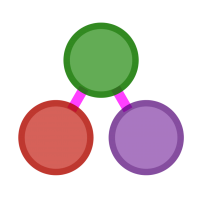
\includegraphics[width=11cm]{juliagraphs.png}}
% \caption{If necessary, the images can be extended both columns.}
%   \label{fig:sample_image}
% \end{figure*}

\section{Additional features}
\label{sec:additional_faci}
In addition to all the standard \LaTeX{} design elements, the \verb|juliacon|  class file includes the following features:
In general, once you have used the additional \verb|juliacon.cls| facilities
in your document, do not process it with a standard \LaTeX{} class
file.

\subsection{Titles, Author's Name, and Affiliation}
\label{subsub:title_auth}
The title of the article, author's name, and affiliation are used at the
beginning of the article (for the main title). These can be produced
using the following code:

\begin{verbatim}
\title{ This is an example of article title} }
\author{
   \large 1st Author \\[-3pt]
   \normalsize 1st author's affiliation  \\[-3pt]
    \normalsize 1st line of address \\[-3pt]
    \normalsize 2nd line of address \\[-3pt]
    \normalsize	1st author's email address \\[-3pt]
  \and
   \large 2nd Author \\[-3pt]
   \normalsize 2nd author's affiliation  \\[-3pt]
    \normalsize 1st line of address \\[-3pt]
    \normalsize 2nd line of address \\[-3pt]
    \normalsize	2nd author's email address \\[-3pt]
\and
   \large 3rd Author \\[-3pt]
   \normalsize 3rd author's affiliation  \\[-3pt]
    \normalsize 1st line of address \\[-3pt]
    \normalsize 2nd line of address \\[-3pt]
    \normalsize	3rd author's email address \\[-3pt]
}
\maketitle
\end{verbatim}

\subsection{Writing Julia code}

A special environment is already defined for Julia code,
built on top of \textit{listings} and \textit{jlcode}.

\begin{verbatim}
\begin{lstlisting}[
    language = Julia, 
    numbers=left, 
    label={lst:exmplg}, 
    caption={Example Code Block.}
]
using Plots

x = -3.0:0.01:3.0
y = rand(length(x))
plot(x, y)
\end{lstlisting}
\end{verbatim}
\begin{lstlisting}[
    language = Julia, 
    numbers=left, 
    label={lst:exmplg}, 
    caption={Example Code Block.}
]
using Plots

x = -3.0:0.01:3.0
y = rand(length(x))
plot(x, y)
\end{lstlisting}


\subsection{Abstracts, Key words, term etc...}
\label{subsub:abs_key_etc}

At the beginning of your article, the title should be generated
in the usual way using the \verb|\maketitle|  command. For genaral tem and keywords use
\verb|\terms|,
\verb|\keywords|  commands respectively. The abstract should be enclosed
within an abstract environment, All these environment
can be produced using the following code:
\begin{verbatim}
\terms{Experimentation, Human Factors}

\keywords{Face animation, image-based modelling...}

\begin{abstract}
In this paper, we propose a new method for the
systematic determination of the model's base of
time varying delay system. This method based on
the construction of the classification data related
to the considered system. The number, the orders,
the time delay and the parameters of the local
models are generated automatically without any
knowledge about the full operating range of the
process. The parametric identification of the local
models is realized by a new recursive algorithm for
on line identification of systems with unknown time
delay. The proposed algorithm allows simultaneous
estimation of time delay and parameters of
discrete-time systems. The effectiveness of
the new method has been illustrated through
simulation.
\end{abstract}

\end{verbatim}

\section{Some guidelines}
\label{sec:some_guide}
The following notes may help you achieve the best effects with the
\verb|juliacon|  class file.

\subsection{Sections}
\label{subsub:sections}
\LaTeXe{}  provides four levels of section headings and they are all
defined in the \verb|juliacon|  class file:
\begin{itemize}
\item \verb|\section|
\item \verb|\subsection|
\item \verb|\subsubsection|
\item \verb|\paragraph|
\end{itemize}
Section headings are automatically converted to allcaps style.
\subsection{Lists}
\label{sec:lists}
%
The \verb|juliacon|   class file provides unnumbered lists using the
\verb|unnumlist|  environment for example,

\begin{unnumlist}
\item First unnumbered item which has no label and is indented from the
left margin.
\item Second unnumbered item.
\item Third unnumbered item.
\end{unnumlist}
The unnumbered list which has no label and is indented from the
left margin. was produced by:
\begin{verbatim}
\begin{unnumlist}
\item First unnumbered item...
\item Second unnumbered item...
\item Third unnumbered item...
\end{unnumlist}
\end{verbatim}

The \verb|juliacon|  class file also provides hyphen list using the
\verb|itemize|  environment for example,
\begin{itemize}
\item First unnumbered bulleted item which has no label and is indented
from the left margin.
\item Second unnumbered bulleted item.
\item Third unnumbered bulleted item which has no label and is indented
from the left margin.
\end{itemize}
was produced by:
\begin{verbatim}
\begin{itemize}
\item First item...
\item Second item...
\item Third item...
\end{itemize}
\end{verbatim}

Numbered list is also provided in acmtog class file using the
enumerate environment for example,
\begin{enumerate}
\item The attenuated and diluted stellar radiation.
\item Scattered radiation, and
\item Reradiation from other grains.
\end{enumerate}

was produced by:
\begin{verbatim}
\begin{enumerate}
\item The attenuated...
\item Scattered radiation, and...
\item Reradiation from other grains...
\end{enumerate}
\end{verbatim}
\subsection{Illustrations (or figures)}
\label{subsub:sec_Illus}
The \verb|juliacon|  class file will cope with most of the positioning of
your illustrations and you should not normally use the optional positional
qualifiers on the \verb|figure|  environment that would override
these decisions.
\vskip 6pt

%
\begin{figure}[t]
\centerline{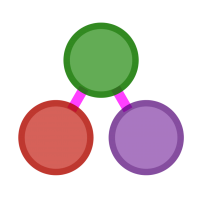
\includegraphics[width=4cm]{juliagraphs.png}}
\caption{This is example of the image in a column.}
	\label{fig:sample_figure}
\end{figure}

The figure \ref{fig:sample_figure} is taken from the JuliaGraphs
organization \footnote{https://github.com/JuliaGraphs}.

Figure captions should be \emph{below} the figure itself, therefore the
\verb|\caption|  command should appear after the figure or space left for
an illustration. For example, Figure 1 is produced using the following
commands:

\begin{verbatim}
\begin{figure}
\centerline{\includegraphics[width=20pc]{Graphics.eps}}
\caption{An example of the testing process for a
binary tree. The globa null hypothesis is tested
first at level $\alpha$ (a), and the level of
individual variables is reached last (d). Note
that individual hypotheses can be tested at
level $\alpha/4$ and not $\alpha/8$ as one might
expect at first.}
\label{sample-figure_2}
\end{figure}
\end{verbatim}
Figures can be resized using first and second argument of
\verb|\includegraphics|   command. First argument is used for modifying
figure height and the second argument is used for modifying
figure width respectively.
\vskip 6pt
Cross-referencing of figures, tables, and numbered, displayed
equations using the \verb|\label|  and \verb|\ref|   commands is encouraged.
For example, in referencing Figure 1 above, we used
\verb|Figure~\ref{sample-figure}|

 \subsection{Tables}
\label{subsub:sec_Tab}
The \verb|juliacon|   class file will cope with most of the positioning of
your tables and you should not normally use the optional positional qualifiers on the table environment which would override these
decisions. Table captions should be at the top.
\begin{verbatim}
\begin{table}
\tbl{Tuning Set and Testing Set}{
\begin{tabular}{|l|l|c|c|}\hline
Label & \multicolumn{1}{c|}{Description}
& Number of Users &
Number of Queries\\\hline
Train70 & Training Data &
\smash{\raise-7pt\hbox{70}} & 104\\
\cline{1-2}\cline{4-4}
Test70 & Testing Data I & & 105\\\hline
Test30 & Testing Data II & 30 & 119\\\hline
& Total & 100 & 328\\\hline
\end{tabular}}
\end{table}
\end{verbatim}

\begin{table}
\tbl{Tuning Set and Testing Set}{
\begin{tabular}{|l|l|c|c|}\hline
Label & \multicolumn{1}{c|}{Description}
& Number of Users &
Number of Queries\\\hline
Test 1 & Training Data &
\smash{\raise-7pt\hbox{70}} & 104\\
\cline{1-2}\cline{4-4}
Test 2 & Testing Data I & & 105\\\hline
Test 3 & Testing Data II & 30 & 119\\\hline
& Total & 100 & 328\\\hline
\end{tabular}}
\end{table}
\subsection{Landscaping Pages}
\label{subsub:landscaping_pages}
If a table is too wide to fit the standard measure, it may be turned,
with its caption, to 90 degrees. Landscape tables cannot be produced
directly using the \verb|juliacon|   class file because \TeX{} itself cannot
turn the page, and not all device drivers provide such a facility.
The following procedure can be used to produce such pages.
\vskip 6pt
Use the package \verb|rotating|   in your document and change the coding
from
\begin{verbatim}
\begin{table}...\end{table}
to
\begin{sidewaystable}...\end{sidewaystable}
and for figures
\begin{figure}...\end{figure}
to
\begin{sidewaysfigure}...\end{sidewaysfigure}
\end{verbatim}

environments in your document to turn your table on the appropriate
page of your document. For instance, the following code prints
a page with the running head, a message half way down and the
table number towards the bottom.
\begin{verbatim}
\begin{sidewaystable}
\tbl{Landscape table caption to go here.}{...}
\label{landtab}
\end{sidewaystable}
\end{verbatim}

\subsection{Double Column Figure and Tables}
\label{subsub:double_fig_tab}
For generating the output of figures and tables in double column
we can use the following coding:

\begin{enumerate}
\item For Figures:
\begin{verbatim}
\begin{figure*}...\end{figure*}
\end{verbatim}
\item For landscape figures:
\begin{verbatim}
\begin{sidewaysfigure*}...\end{sidewaysfigure*}
\end{verbatim}
\item For Tables:
\begin{verbatim}
\begin{table*}...\end{table*}
\end{verbatim}
\item For landscape tables:
\begin{verbatim}
\begin{sidewaystable*}...\end{sidewaystable*}
\end{verbatim}
\end{enumerate}

\subsection{Typesetting Mathematics}
\label{subsub:type_math}
The \verb|juliacon| class file will set displayed mathematics with center to
the column width, provided that you use the \LaTeXe{} standard of
open and closed square brackets as delimiters.
The equation
\[
\sum_{i=1}^p \lambda_i = (S)
\]

was typeset using the acmtog class file with the commands

\begin{verbatim}
\[
\sum_{i=1}^p \lambda_i = (S)
\]
\end{verbatim}

For display equations, cross-referencing is encouraged. For example,
\begin{verbatim}
\begin{equation}
(n-1)^{-1} \sum^n_{i=1} (X_i - \overline{X})^2.
\label{eq:samplevar}
\end{equation}
Equation~(\ref{eq:samplevar}) gives the formula for
sample variance.
\end{verbatim}
The following output is generated with the above coding:
\begin{equation}
(n-1)^{-1} \sum^n_{i=1} (X_i - \overline{X})^2.
\label{eq:samplevar}
\end{equation}
Equation~(\ref{eq:samplevar}) gives the formula for
sample variance.


\subsection{Enunciations}
\label{subsub:enunciation}
The \verb|juliacon|   class file generates the enunciations with the help of
the following commands:
\begin{verbatim}
\begin{theorem}...\end{theorem}
\begin{strategy}...\end{strategy}
\begin{property}...\end{property}
\begin{proposition}...\end{proposition}
\begin{lemma}...\end{lemma}
\begin{example}...\end{example}
\begin{proof}...\end{proof}
\begin{definition}...\end{definition}
\begin{algorithm}...\end{algorithm}
\begin{remark}...\end{remark}
\end{verbatim}
The above-mentioned coding can also include optional arguments
such as
\begin{verbatim}
\begin{theorem}[...]. Example for theorem:
\begin{theorem}[Generalized Poincare Conjecture]
Four score and seven ... created equal.
\end{theorem}
\end{verbatim}

\begin{theorem}[Generalized Poincare Conjecture]
Four score and seven years ago our fathers brought forth,
upon this continent, a new nation, conceived in Liberty,
 and dedicated to the proposition that all men are
created equal.
\end{theorem}


\subsection{Extract}
\label{subsub:extract}
Extract environment should be coded within
\begin{verbatim}
\begin{extract}..\end{extract}
\end{verbatim}

\subsection{Balancing column at last page}
\label{subsub:Balance}
For balancing the both column length at last page use :
\begin{verbatim}
\vadjust{\vfill\pagebreak}
\end{verbatim}

%\vadjust{\vfill\pagebreak}

at appropriate place in your \TeX{} file or in bibliography file.

\section{Handling references}
\label{subsub:references}
References are most easily (and correctly) generated using the
BIBTEX, which is easily invoked via
\begin{verbatim}
\bibliographystyle{juliacon}
\bibliography{ref}
\end{verbatim}
When submitting the document source (.tex) file to external
parties, the ref.bib file should be sent with it.
\cite{bezanson2017julia}

\section{Acknowledgements}

B. S. Flores would like to acknowledge the members of the geometric algebra community at bivector.net.
Specifically, this includes David Cohoe (sudgylacmoe), Steven de Keninck (enki), Hamish Todd, and Moab Croft (Slackline).
B. S. Flores would also like to acknowledge Chris Doran and Cédric Belmant (serenity7) for discussing the implementation of Clifford algebras in Julia, as well as Mateusz Baran for discussion of the related StaticArrays.jl package.
Finally, B. S. Flores would like to acknowledge Dr. Michael Davies for bringing him an appreciation for computing on all levels, from hardware to the human.

\input{bib.tex}

\end{document}

% Inspired by the International Journal of Computer Applications template
